\documentclass[aspectratio=169,10pt]{beamer}

\usepackage{ctex}
\usepackage[T1]{fontenc}
\usepackage{amsmath,booktabs,array,colortbl,tabularx}
\usepackage{graphicx}
\usepackage{tikz}
\usetikzlibrary{arrows.meta,positioning,calc}
\usepackage{SoutheastUniversity}

\author{夏秋桐}
\title{GearPro 齿轮视觉检测系统阶段汇报}
\subtitle{软件视觉系统阶段进展}
\date{2026-09-28}
\titlegraphic{
\includegraphics[width=.145\paperwidth]{pic/Southeast_University_Logo.pdf}}

\newcommand{\OverviewNav}{%
  \GearProSetMajor{总览}%
  \GearProHideMinorNav%
}

\newcommand{\SoftwareNav}[1]{%
  \GearProSetMajor{软件}%
  \GearProSetMinorNavFive{阶段现状}{流程与数据}{架构决策}{双专项}{结果分析}{#1}%
}

\newcommand{\smallnote}[1]{%
  \par\vspace{.35em}{\scriptsize\color{seugray}#1}%
}

\tikzset{
  flow/.style={draw=seugreen,very thick,rounded corners=2pt,fill=seugreenlight,
    align=center,minimum height=1.05cm,text width=2.2cm,inner sep=5pt},
  flowwide/.style={flow,text width=2.75cm},
  decision/.style={draw=seugold,very thick,rounded corners=2pt,fill=seuyellowlight,
    align=center,minimum height=1.05cm,text width=2.15cm,inner sep=5pt},
  line/.style={-{Latex[length=2.2mm]},very thick,draw=seugreen}
}

\begin{document}

% 1. Cover
\begin{frame}[plain]
  \titlepage
\end{frame}

% 2. Outline
\OverviewNav
\begin{frame}{汇报结构}
  \vspace{.25em}
  \begin{columns}[T,onlytextwidth]
    \begin{column}{.32\textwidth}
      \begin{block}{软件}
        \textbf{本轮完整汇报}

        \vspace{.45em}
        任务、数据、架构、双专项、结果与错误分析
      \end{block}
    \end{column}
    \begin{column}{.32\textwidth}
      \begin{exampleblock}{硬件}
        \textbf{后续补充}

        \vspace{.45em}
        平台目标、相机与载台、照明、视角和实验验证
      \end{exampleblock}
    \end{column}
    \begin{column}{.32\textwidth}
      \begin{exampleblock}{联合}
        \textbf{后续补充}

        \vspace{.45em}
        软硬件接口、端到端验收和阶段结论
      \end{exampleblock}
    \end{column}
  \end{columns}

  \vfill
  \centering
  \textcolor{seugreen}{\large 本轮重点说明软件路线为何形成，以及当前误差指向哪里}
\end{frame}

% 3. Overall status
\begin{frame}{项目阶段总述}
  \begin{columns}[T,onlytextwidth]
    \begin{column}{.3\textwidth}
      \centering
      {\color{seugreen}\LARGE\bfseries 软件}

      \vspace{.5em}
      输入、推理、判定、统计、Web 与串口已经连通
    \end{column}
    \begin{column}{.04\textwidth}
      \centering\vspace{1.2em}{\color{seugold}\Large$+$}
    \end{column}
    \begin{column}{.3\textwidth}
      \centering
      {\color{seugreen}\LARGE\bfseries 硬件}

      \vspace{.5em}
      相机、载台、照明和补充视角仍需实验定型
    \end{column}
    \begin{column}{.04\textwidth}
      \centering\vspace{1.2em}{\color{seugold}\Large$=$}
    \end{column}
    \begin{column}{.3\textwidth}
      \centering
      {\color{seugreen}\LARGE\bfseries 联合}

      \vspace{.5em}
      最终从原始相机帧开始验收 Recall、FPR 与运行稳定性
    \end{column}
  \end{columns}

  \vfill
  \begin{alertblock}{当前边界}
    离线锁定测试用于比较方案，不能替代真实相机、照明、传送结构和执行机构条件下的端到端结果。
  \end{alertblock}
\end{frame}

\section{软件}

% 4. Current state
\subsection{阶段现状}
\SoftwareNav{1}
\begin{frame}{软件阶段现状}
  \begin{columns}[T,onlytextwidth]
    \begin{column}{.46\textwidth}
      \textbf{已实现}
      \begin{itemize}
        \item Model1 定位与 4\% ROI 外扩
        \item Scratch V5 与 Missing Hole V1
        \item 独立阈值、最终 OR 与拒绝原因
        \item Web 控制台、统计和串口输出
        \item 模型哈希校验与有限安全停机
      \end{itemize}

      \vspace{.25em}
      \textbf{仍待验收}
      \begin{itemize}
        \item Jetson NX 的延迟、功耗和稳定性
        \item 真实结构与照明下的端到端指标
      \end{itemize}
    \end{column}
    \begin{column}{.51\textwidth}
      \centering
      % TODO: replace with the original high-resolution screenshot when available.
      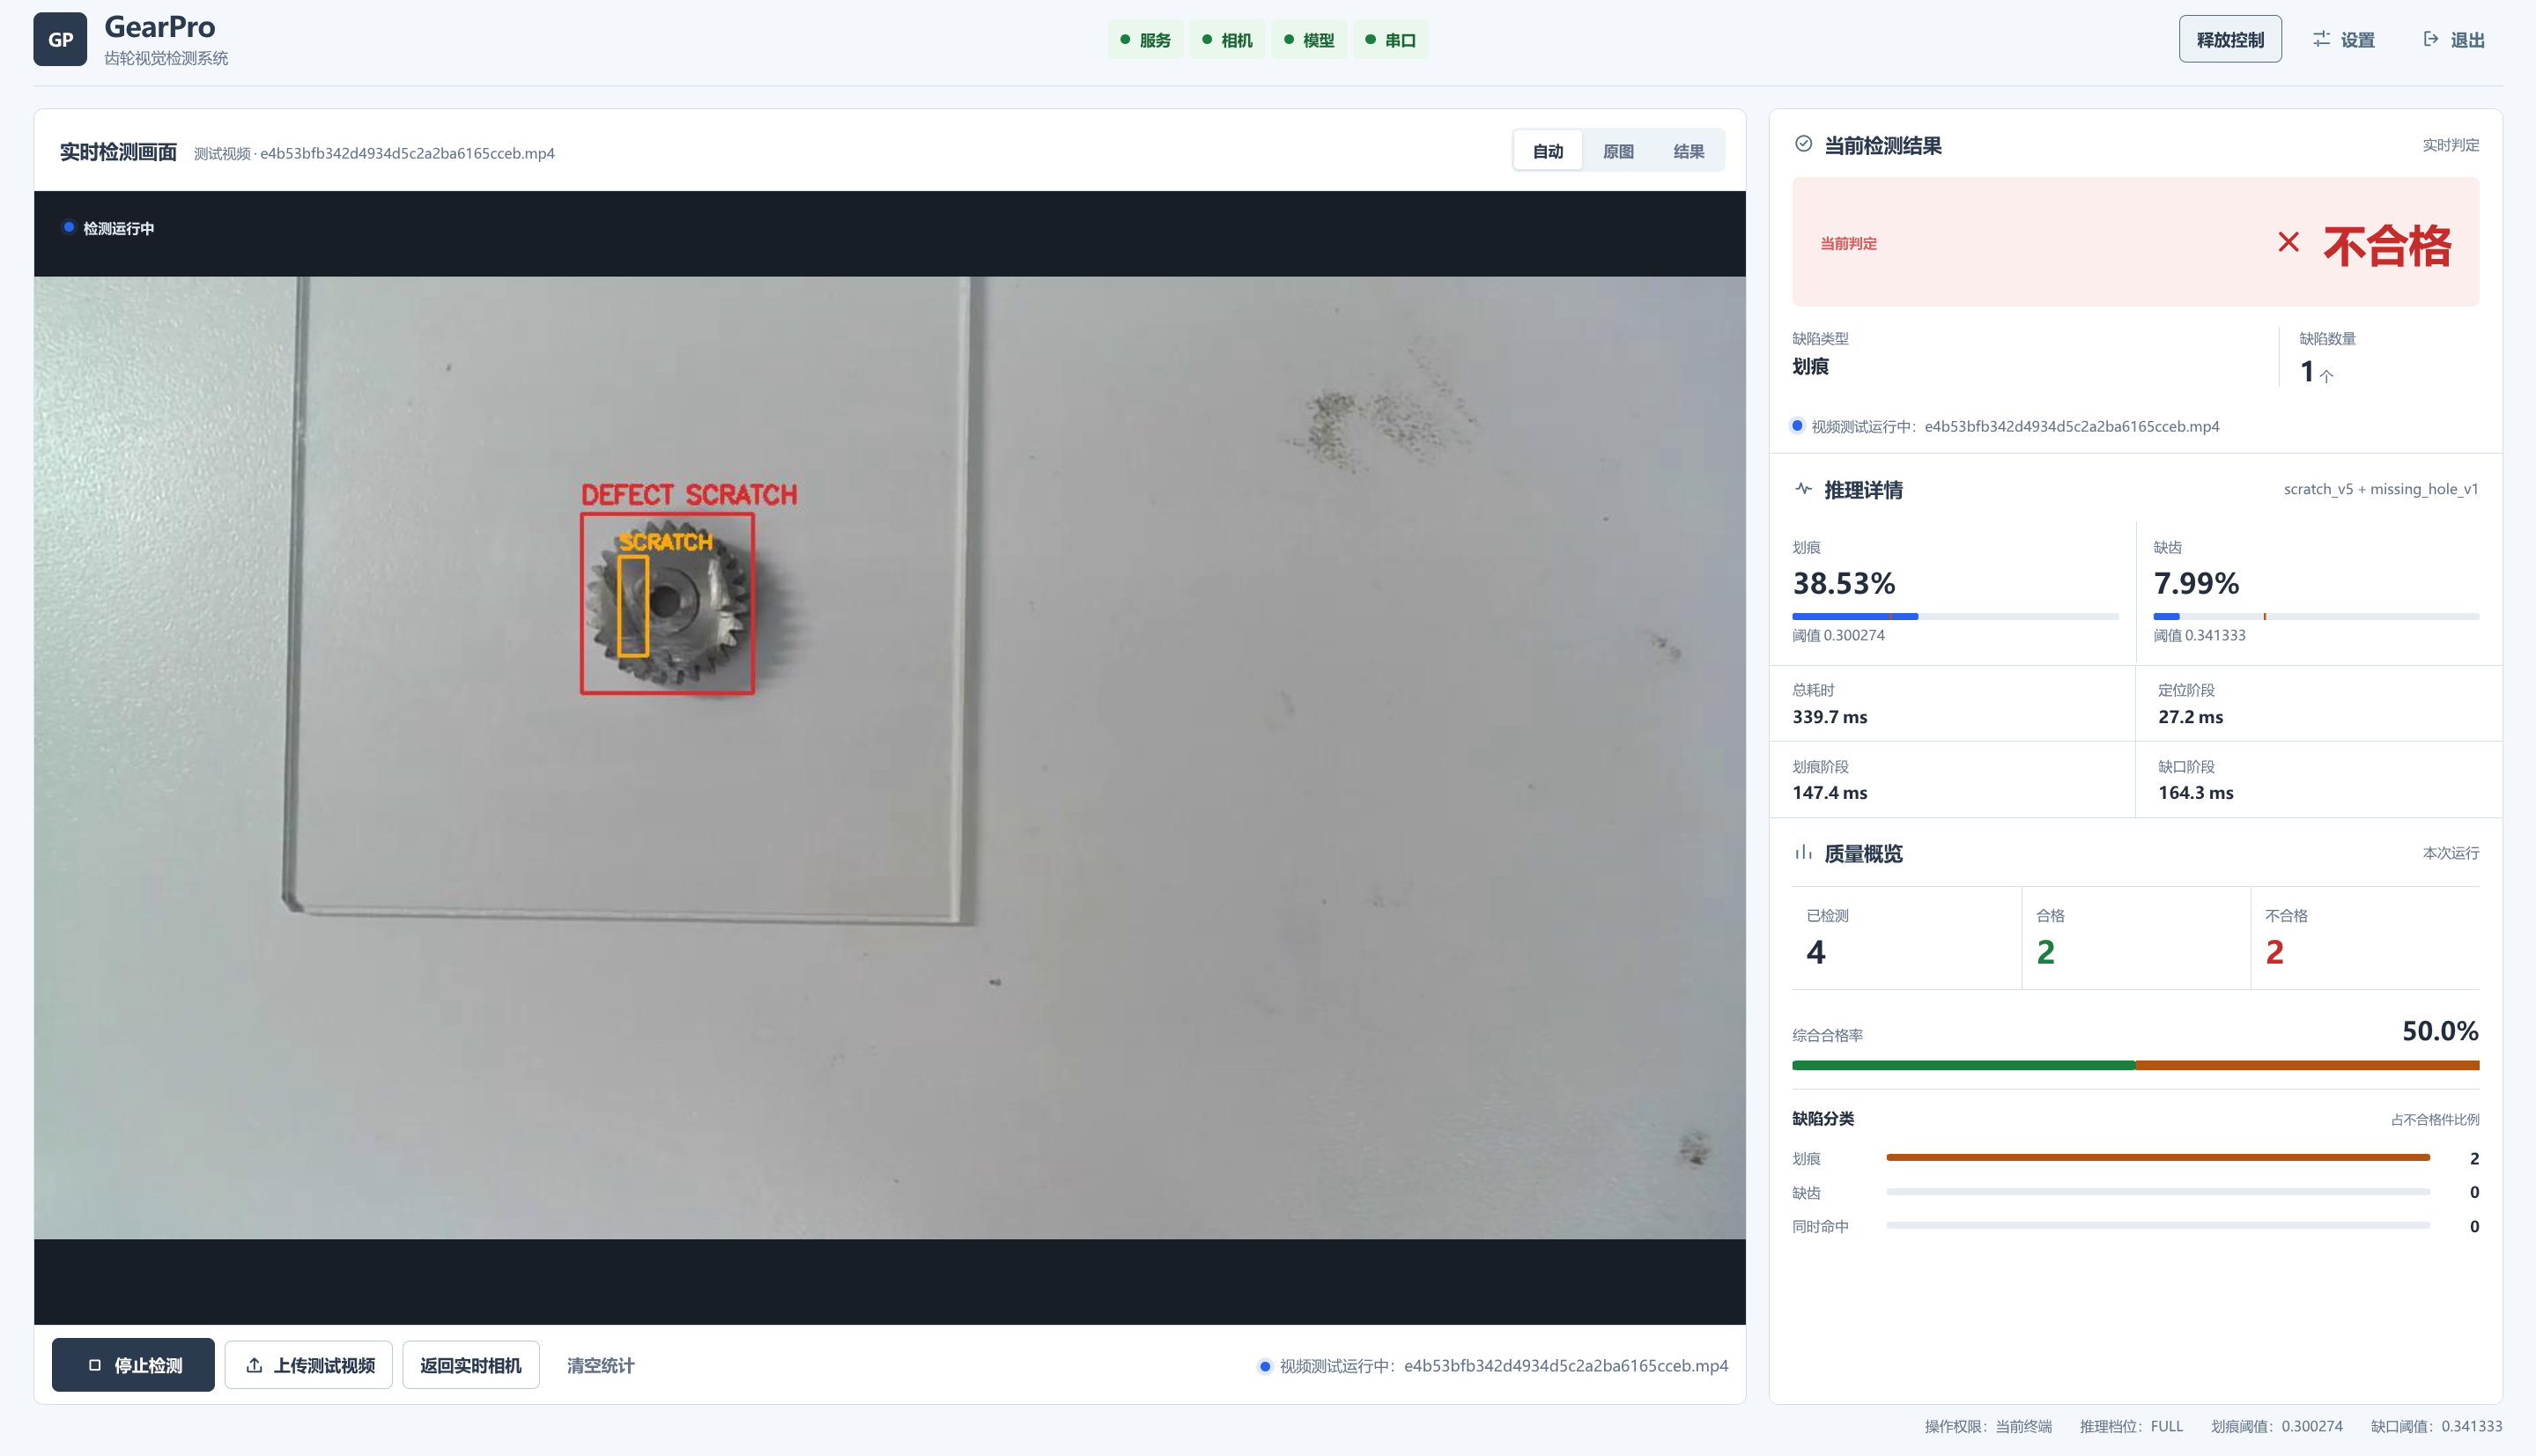
\includegraphics[width=\linewidth,height=.61\textheight,keepaspectratio]{pic/gearpro/web_console.png}
      \smallnote{现有 Web 控制台截图，后续可替换原始高分辨率版本}
    \end{column}
  \end{columns}

  \vfill
  \centering
  \textcolor{seugreen}{\large 结论：软件闭环已运行，模型和真实设备尚未完成生产验收}
\end{frame}

% 5. Tasks and metrics
\begin{frame}{任务与评价标准}
  \begin{columns}[T,onlytextwidth]
    \begin{column}{.49\textwidth}
      \textbf{三个视觉任务}
      \begin{description}
        \item[定位] Model1 判断齿轮在哪里，并产生 ROI
        \item[划痕] 识别低对比、局部纹理型缺陷
        \item[缺口] 识别齿形和轮廓的结构变化
      \end{description}

      \vspace{.5em}
      \begin{exampleblock}{端到端口径}
        Model1 漏定位、ROI 偏移和输出链路失败都必须计入最终结果。
      \end{exampleblock}
    \end{column}
    \begin{column}{.47\textwidth}
      \renewcommand{\arraystretch}{1.35}
      \begin{tabularx}{\linewidth}{>{\bfseries\color{seugreen}}l X}
        Recall & 真实缺陷中被检出的比例，反映漏检风险 \\
        FPR & 正常样本被误判为缺陷的比例，反映误剔除风险 \\
        Precision & 判为缺陷的结果中真正缺陷的比例 \\
        mAP & 辅助框质量，不直接等于工件判定能力 \\
      \end{tabularx}

      \vspace{.8em}
      \centering
      {\color{seugreen}\large\bfseries 阶段目标}

      \vspace{.25em}
      {\Large Recall $\geq 0.95$}\qquad
      {\Large FPR $\leq 0.20$}
    \end{column}
  \end{columns}
\end{frame}

% 6. Pipeline
\subsection{流程与数据}
\SoftwareNav{2}
\begin{frame}{当前视觉处理流程}
  \centering
  \resizebox{.96\textwidth}{!}{%
    \begin{tikzpicture}[node distance=.65cm and .6cm]
      \node[flow] (input) {相机或\\测试视频};
      \node[flow,right=of input] (loc) {Model1\\齿轮定位};
      \node[flow,right=of loc] (roi) {定位框外扩 4\%\\裁剪 ROI};
      \node[flowwide,right=of roi] (spec) {Scratch V5\\Missing Hole V1};
      \node[decision,right=of spec] (judge) {各自校准\\独立过阈值};
      \node[decision,right=of judge] (or) {最终 OR\\合格或剔除};
      \draw[line] (input) -- (loc);
      \draw[line] (loc) -- (roi);
      \draw[line] (roi) -- (spec);
      \draw[line] (spec) -- (judge);
      \draw[line] (judge) -- (or);
    \end{tikzpicture}%
  }

  \vspace{1.0em}
  \begin{columns}[T,onlytextwidth]
    \begin{column}{.31\textwidth}
      \textbf{多个齿轮}

      逐个生成 ROI，任意齿轮命中任意专项，整帧判为不合格。
    \end{column}
    \begin{column}{.31\textwidth}
      \textbf{没有齿轮}

      不计数，不发送串口结果，避免无效输出。
    \end{column}
    \begin{column}{.31\textwidth}
      \textbf{测试视频}

      主动禁用串口，防止测试素材触发真实执行机构。
    \end{column}
  \end{columns}

  \vfill
  \centering
  同一推理结果同时进入 \textbf{Web、统计和串口}，各模块不重复计算判定。
\end{frame}

% 7. Data split
\begin{frame}{数据拆分与锁定测试}
  \centering
  \begin{tikzpicture}[node distance=1.15cm]
    \node[flowwide] (train) {训练集\\更新模型参数};
    \node[flowwide,right=of train] (val) {验证集\\选择结构、校准与阈值};
    \node[decision,right=of val] (test) {锁定测试\\配置冻结后只使用一次};
    \draw[line] (train) -- (val);
    \draw[line] (val) -- (test);
  \end{tikzpicture}

  \vspace{1em}
  \begin{columns}[T,onlytextwidth]
    \begin{column}{.48\textwidth}
      \textbf{为什么不能随机按图片拆分}
      \begin{itemize}
        \item 连续帧和相近角度高度相似
        \item 同一工件纹理可能跨集合出现
        \item 验证分数会虚高
      \end{itemize}
    \end{column}
    \begin{column}{.48\textwidth}
      \textbf{当前隔离方法}
      \begin{itemize}
        \item SHA256 检查精确重复
        \item dHash 发现视觉近似项
        \item 结合序号、宽高比和灰度相关性建组
        \item 同组不跨训练、验证和测试集合
      \end{itemize}
    \end{column}
  \end{columns}

  \vfill
  \begin{alertblock}{测试纪律}
    查看锁定测试结果后，不能再依据该测试集修改温度、融合权重或阈值。
  \end{alertblock}
\end{frame}

% 8. Difficult labels
\begin{frame}{Difficult 标签治理}
  \begin{columns}[T,onlytextwidth]
    \begin{column}{.46\textwidth}
      \begin{block}{include 训练口径}
        保留 difficult 框，让训练集包含全部已标注缺陷。
      \end{block}

      \vspace{.55em}
      \begin{block}{exclude 训练口径}
        删除 difficult 框；若一张图片只剩 difficult 缺陷，则整张图片退出训练。
      \end{block}
    \end{column}
    \begin{column}{.49\textwidth}
      \textbf{必须避免的错误}

      \vspace{.5em}
      \begin{alertblock}{假负样本}
        删除缺陷框后继续把图片当作正常样本，会让模型把真实缺陷学习成正常外观。
      \end{alertblock}

      \vspace{.55em}
      \textbf{统一评价}
      \begin{itemize}
        \item 验证集和测试集保留完整真值
        \item 不同训练策略使用同一评价口径
        \item 结果显示 oblique 视角才是主要瓶颈
      \end{itemize}
    \end{column}
  \end{columns}

  \vfill
  \centering
  \textcolor{seugreen}{\large 数据治理同时控制图像泄漏和标签语义污染}
\end{frame}

% 9. ROI
\subsection{架构决策}
\SoftwareNav{3}
\begin{frame}{关键决策一：先定位，再识别缺陷}
  \begin{columns}[T,onlytextwidth]
    \begin{column}{.45\textwidth}
      \centering
      \begin{tikzpicture}
        \node[flowwide,minimum height=2.1cm] (full) {整帧缩放\\背景占用像素预算\\微小划痕继续缩小};
        \node[decision,below=1.0cm of full,minimum height=1.55cm] (loss) {连续下采样后\\缺陷可能不足有效网格};
        \draw[line] (full) -- (loss);
      \end{tikzpicture}
    \end{column}
    \begin{column}{.08\textwidth}
      \centering\vspace{2.4em}{\color{seugold}\Huge$\Rightarrow$}
    \end{column}
    \begin{column}{.45\textwidth}
      \centering
      \begin{tikzpicture}
        \node[flowwide,minimum height=2.1cm] (loc) {Model1 定位\\宽高方向各外扩 4\%};
        \node[flowwide,below=1.0cm of loc,minimum height=1.55cm] (roi) {高分辨率 ROI\\保留齿轮表面与边缘上下文};
        \draw[line] (loc) -- (roi);
      \end{tikzpicture}
    \end{column}
  \end{columns}

  \vfill
  \begin{columns}[T,onlytextwidth]
    \begin{column}{.48\textwidth}
      \textbf{收益：}减少背景和姿态干扰，把输入分辨率集中到齿轮区域。
    \end{column}
    \begin{column}{.48\textwidth}
      \textbf{边界：}Model1 漏定位仍属于端到端漏检，4\% 外扩需要真实设备继续验证。
    \end{column}
  \end{columns}
\end{frame}

% 10. Unified versus specialists
\begin{frame}{关键决策二：统一模型转向双专项}
  \begin{columns}[T,onlytextwidth]
    \begin{column}{.43\textwidth}
      \centering
      {\large\bfseries 统一模型}

      \vspace{.7em}
      \begin{tabular}{lr}
        Recall & 0.7606 \\
        FPR & 0.4177 \\
      \end{tabular}

      \vspace{1.0em}
      同时学习微小纹理和结构缺口，当前数据下监督信号分散。
    \end{column}
    \begin{column}{.12\textwidth}
      \centering\vspace{2em}{\color{seugold}\Huge$\Rightarrow$}
    \end{column}
    \begin{column}{.43\textwidth}
      \centering
      {\large\bfseries 双专项 OR}

      \vspace{.7em}
      \begin{tabular}{lr}
        Recall & \textbf{0.8873} \\
        FPR & \textbf{0.2278} \\
      \end{tabular}

      \vspace{1.0em}
      两类缺陷分别选择输入、检测头、概率校准和发布阈值。
    \end{column}
  \end{columns}

  \vfill
  \begin{block}{拆分依据}
    划痕表现为小面积、低对比纹理变化；缺齿缺口表现为轮廓和结构变化。当前结果支持专项化，但不排除未来在更多数据下重新评估统一模型。
  \end{block}
\end{frame}

% 11. Scratch architecture
\subsection{双专项}
\SoftwareNav{4}
\begin{frame}{Scratch V5：整体分类与局部检测互补}
  \centering
  \resizebox{.92\textwidth}{!}{%
    \begin{tikzpicture}[node distance=.55cm and .65cm]
      \node[flowwide] (roi) {齿轮 ROI};
      \node[flowwide,above right=.15cm and 1.2cm of roi] (eff) {EfficientNet-B0\\384 输入};
      \node[flowwide,right=1.2cm of roi] (res) {ResNet18\\384 输入};
      \node[flowwide,below right=.15cm and 1.2cm of roi] (det) {YOLO26-P2\\960 输入};
      \node[decision,right=1.25cm of res] (cal) {逐路温度校准};
      \node[decision,right=1.0cm of cal] (fuse) {专项融合概率};
      \draw[line] (roi) -- (eff);
      \draw[line] (roi) -- (res);
      \draw[line] (roi) -- (det);
      \draw[line] (eff.east) -- (cal.west);
      \draw[line] (res) -- (cal);
      \draw[line] (det.east) -- (cal.west);
      \draw[line] (cal) -- (fuse);
    \end{tikzpicture}%
  }

  \vspace{.7em}
  \begin{exampleblock}{发布公式}
    \centering
    $p_{\mathrm{scratch}} = 0.25\,p_{\mathrm{cls}} + 0.75\,p_{\mathrm{det}}$
    \qquad
    阈值 $= 0.300273610279458$
  \end{exampleblock}

  \vfill
  \begin{columns}[T,onlytextwidth]
    \begin{column}{.48\textwidth}
      分类器判断整张 ROI 的整体外观，P2 检测器强化细小局部划痕。
    \end{column}
    \begin{column}{.48\textwidth}
      弱检测概率参与融合；辅助框使用更高显示门槛，只服务人工复核。
    \end{column}
  \end{columns}
\end{frame}

% 12. Scratch result
\begin{frame}{Scratch V5 锁定测试结果}
  \begin{columns}[T,onlytextwidth]
    \begin{column}{.39\textwidth}
      \centering
      % TODO: replace with the original high-resolution scratch image when available.
      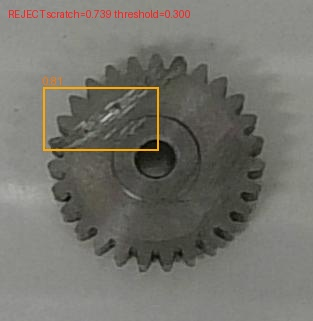
\includegraphics[width=.82\linewidth,height=.59\textheight,keepaspectratio]{pic/gearpro/scratch_reject.jpg}
      \smallnote{现有划痕检测示例}
    \end{column}
    \begin{column}{.57\textwidth}
      \begin{columns}[T,onlytextwidth]
        \begin{column}{.32\textwidth}
          \centering {\color{seugreen}\LARGE\bfseries 0.8065}\\Recall
        \end{column}
        \begin{column}{.32\textwidth}
          \centering {\color{seugreen}\LARGE\bfseries 0.5556}\\Precision
        \end{column}
        \begin{column}{.32\textwidth}
          \centering {\color{seugreen}\LARGE\bfseries 0.1681}\\FPR
        \end{column}
      \end{columns}

      \vspace{1.0em}
      \centering
      \begin{tabular}{ccccc}
        \toprule
        样本 & TP & FP & TN & FN \\
        \midrule
        150 & 25 & 20 & 99 & 6 \\
        \bottomrule
      \end{tabular}

      \vspace{1em}
      \begin{itemize}
        \item FN：低对比、小面积或外观不稳定划痕
        \item FP：侧齿高光和正常加工纹
      \end{itemize}
    \end{column}
  \end{columns}

  \vfill
  \centering
  \textcolor{seugreen}{检测器增强局部敏感性，但高光与加工纹仍限制泛化}
\end{frame}

% 13. Missing architecture
\begin{frame}{Missing Hole V1：结构缺陷专项}
  \centering
  \resizebox{.92\textwidth}{!}{%
    \begin{tikzpicture}[node distance=.55cm and .65cm]
      \node[flowwide] (roi) {齿轮 ROI};
      \node[flowwide,above right=.15cm and 1.2cm of roi] (eff) {EfficientNet-B0\\512 输入};
      \node[flowwide,right=1.2cm of roi] (res) {ResNet18\\384 输入};
      \node[flowwide,below right=.15cm and 1.2cm of roi] (det) {标准 YOLO26n\\960 输入};
      \node[decision,right=1.25cm of res] (cal) {逐路温度校准};
      \node[decision,right=1.0cm of cal] (fuse) {专项融合概率};
      \draw[line] (roi) -- (eff);
      \draw[line] (roi) -- (res);
      \draw[line] (roi) -- (det);
      \draw[line] (eff.east) -- (cal.west);
      \draw[line] (res) -- (cal);
      \draw[line] (det.east) -- (cal.west);
      \draw[line] (cal) -- (fuse);
    \end{tikzpicture}%
  }

  \vspace{.7em}
  \begin{exampleblock}{发布公式}
    \centering
    $p_{\mathrm{missing}} = 0.50\,p_{\mathrm{cls}} + 0.50\,p_{\mathrm{det}}$
    \qquad
    阈值 $= 0.3413327979078584$
  \end{exampleblock}

  \vfill
  \begin{block}{为什么没有使用 P2}
    P2 在 Missing Hole 验证实验中没有稳定胜过标准检测头。模型结构由任务和数据决定，不能只根据“目标可能较小”直接保留 P2。
  \end{block}
\end{frame}

% 14. Missing result
\begin{frame}{Missing Hole V1 锁定测试结果}
  \begin{columns}[T,onlytextwidth]
    \begin{column}{.36\textwidth}
      \centering
      % TODO: replace with the original high-resolution oblique image when available.
      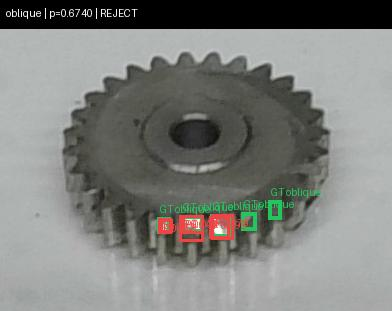
\includegraphics[width=.9\linewidth,height=.54\textheight,keepaspectratio]{pic/gearpro/oblique_missing.jpg}
      \smallnote{oblique 缺口示例}
    \end{column}
    \begin{column}{.6\textwidth}
      \begin{columns}[T,onlytextwidth]
        \begin{column}{.32\textwidth}
          \centering {\color{seugreen}\LARGE\bfseries 0.8182}\\Recall
        \end{column}
        \begin{column}{.32\textwidth}
          \centering {\color{seugreen}\LARGE\bfseries 0.9000}\\Precision
        \end{column}
        \begin{column}{.32\textwidth}
          \centering {\color{seugreen}\LARGE\bfseries 0.0377}\\FPR
        \end{column}
      \end{columns}

      \vspace{.8em}
      \textbf{位置子组 Recall}

      \vspace{.35em}
      \begin{tabular}{lcl}
        bottom & \textcolor{seugreen}{\rule{3.20cm}{1.1ex}} & 0.9167 \\
        side & \textcolor{seugreen}{\rule{3.49cm}{1.1ex}} & 1.0000 \\
        oblique & \textcolor{seugold}{\rule{2.05cm}{1.1ex}} & \textbf{0.5882} \\
      \end{tabular}

      \vspace{.8em}
      TP/FP/TN/FN：36/4/102/8
    \end{column}
  \end{columns}

  \vfill
  \begin{alertblock}{主要瓶颈}
    difficult 统计口径变化很小，oblique 视角下的结构可见性才是当前最明确的问题。
  \end{alertblock}
\end{frame}

% 15. OR decision
\begin{frame}{关键决策三：独立阈值后执行 OR}
  \centering
  \begin{tikzpicture}[node distance=1.1cm and 1.05cm]
    \node[flowwide,text width=3.75cm] (scratch) {Scratch 概率\\{\scriptsize$\geq 0.300273610279458$}};
    \node[flowwide,text width=3.75cm,below=of scratch] (missing) {Missing Hole 概率\\{\scriptsize$\geq 0.3413327979078584$}};
    \coordinate (join) at ($(scratch.east)!0.5!(missing.east)+(0.75cm,0)$);
    \node[decision,right=1.0cm of join] (or) {逻辑 OR};
    \node[flowwide,right=1.25cm of or] (final) {最终结果\\合格或不合格};
    \draw[very thick,draw=seugreen] (scratch.east) -| (join);
    \draw[very thick,draw=seugreen] (missing.east) -| (join);
    \draw[line] (join) -- (or.west);
    \draw[line] (or) -- (final);
  \end{tikzpicture}

  \vspace{1em}
  \begin{columns}[T,onlytextwidth]
    \begin{column}{.47\textwidth}
      \textbf{为什么独立过阈值}

      两个专项的任务、温度校准和概率分布不同，没有证据支持直接相加后使用统一阈值。
    \end{column}
    \begin{column}{.47\textwidth}
      \textbf{OR 的代价}

      可以补回另一专项漏掉的缺陷，也会合并两个专项的误报集合。
    \end{column}
  \end{columns}

  \vfill
  \centering
  同一齿轮同时命中两个专项时保留两个原因，统计和串口只输出一次。
\end{frame}

% 16. Core results
\subsection{结果分析}
\SoftwareNav{5}
\begin{frame}{核心锁定测试结果}
  \centering
  \renewcommand{\arraystretch}{1.3}
  \begin{tabular}{lrrrr}
    \toprule
    方案 & Recall & Precision & FPR & TP/FP/TN/FN \\
    \midrule
    Scratch V5 专项 & 0.8065 & 0.5556 & 0.1681 & 25/20/99/6 \\
    Missing Hole V1 专项 & 0.8182 & 0.9000 & 0.0377 & 36/4/102/8 \\
    \rowcolor{seuyellowlight}
    双专项 OR & \textbf{0.8873} & \textbf{0.7778} & \textbf{0.2278} & 63/18/61/8 \\
    统一 EfficientNet-B0 & 0.7606 & 0.6207 & 0.4177 & 54/33/46/17 \\
    \bottomrule
  \end{tabular}

  \vspace{1.2em}
  \begin{columns}[T,onlytextwidth]
    \begin{column}{.47\textwidth}
      \textbf{同口径结论}

      双专项 OR 相比统一模型提高任意缺陷 Recall，并显著降低 FPR。
    \end{column}
    \begin{column}{.47\textwidth}
      \textbf{不能直接比较的数字}

      两个专项的负样本定义不同，专项 FPR 不能简单相加。
    \end{column}
  \end{columns}

  \vfill
  \centering
  \textcolor{seugreen}{当前方案优于统一模型，但仍未达到生产目标}
\end{frame}

% 17. Target gap
\begin{frame}{目标差距与阈值纪律}
  \begin{columns}[T,onlytextwidth]
    \begin{column}{.48\textwidth}
      \centering
      {\small Recall}

      \vspace{.25em}
      {\color{seugreen}\Huge\bfseries 0.8873}

      \vspace{.15em}
      目标 0.95，仍差 \textbf{0.0627}
    \end{column}
    \begin{column}{.48\textwidth}
      \centering
      {\small FPR}

      \vspace{.25em}
      {\color{seugreen}\Huge\bfseries 0.2278}

      \vspace{.15em}
      上限 0.20，超出 \textbf{0.0278}
    \end{column}
  \end{columns}

  \vspace{1em}
  \begin{alertblock}{不能继续用当前 test 调阈值}
    锁定测试已经参与最终评价。根据其结果重新选择阈值，会破坏测试独立性，并可能用显著增加误报的方式换取表面召回提升。
  \end{alertblock}

  \vfill
  \centering
  下一轮优化应在新数据上完成模型与阈值选择，配置冻结后建立新的 blind test。
\end{frame}

% 18. Error patterns
\begin{frame}{主要错误模式}
  \begin{columns}[T,onlytextwidth]
    \begin{column}{.31\textwidth}
      \textbf{低对比划痕 FN}

      缺陷纹理接近正常加工纹。优先稳定低角度照明，并补采真实弱划痕。
    \end{column}
    \begin{column}{.31\textwidth}
      \textbf{oblique 缺口 FN}

      单一视角下结构变化不稳定。优先验证背光、第二相机或转台。
    \end{column}
    \begin{column}{.31\textwidth}
      \textbf{高光正常样本 FP}

      侧齿反光和加工纹触发划痕分支。需要调整光源并扩充真实负样本。
    \end{column}
  \end{columns}

  \vspace{.85em}
  \centering
  % TODO: replace this montage with original full-resolution error cases when available.
  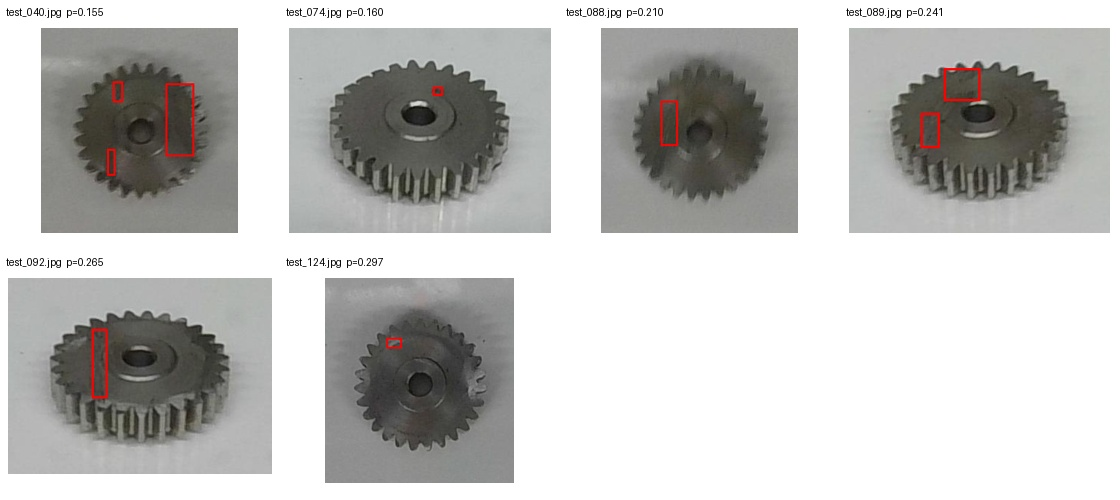
\includegraphics[width=.88\linewidth,height=.42\textheight,keepaspectratio]{pic/gearpro/error_cases.jpg}
  \smallnote{现有错误样本组合图，后续替换为原始单图}
\end{frame}

% 19. Conclusion and transition
\begin{frame}{软件阶段结论}
  \begin{columns}[T,onlytextwidth]
    \begin{column}{.31\textwidth}
      \centering
      {\color{seugreen}\Large\bfseries 实验}

      \vspace{.5em}
      已建立按组隔离、标签治理、锁定测试和 Recall/FPR 双约束。
    \end{column}
    \begin{column}{.31\textwidth}
      \centering
      {\color{seugreen}\Large\bfseries 模型}

      \vspace{.5em}
      已形成 Model1 定位与 Scratch、Missing Hole 双专项方案。
    \end{column}
    \begin{column}{.31\textwidth}
      \centering
      {\color{seugreen}\Large\bfseries 差距}

      \vspace{.5em}
      联合 Recall 0.8873、FPR 0.2278，真实设备结果仍待验收。
    \end{column}
  \end{columns}

  \vspace{1.1em}
  \begin{block}{当前技术判断}
    低对比划痕、oblique 缺口和高光误报都与输入可见性和数据覆盖密切相关。下一阶段应先验证成像条件，再决定模型复杂度。
  \end{block}

  \vfill
  \begin{exampleblock}{下一部分：硬件结构与成像平台}
    重点比较相机工作距离、玻璃载台、背光、低角度表面照明，以及第二相机或转台的新增信息。
  \end{exampleblock}
\end{frame}

\end{document}
